\documentclass[10pt]{article}
\usepackage[T1]{fontenc}
\usepackage{amsmath,amssymb,amsthm,mathtools}
\usepackage{graphicx,microtype}
\usepackage{titlesec}
\usepackage[margin=0.78in]{geometry}
\usepackage[hidelinks]{hyperref}
\titlespacing*{\section}{0pt}{1.5ex plus .4ex minus .2ex}{0.7ex}

\newtheorem{theorem}{Theorem}
\newtheorem{lemma}[theorem]{Lemma}
\newtheorem{remark}[theorem]{Remark}
\newcommand{\R}{\mathbb R}
\newcommand{\vol}{\operatorname{vol}}

\title{Cartesian products disprove asymptotic cube optimality\\
\large A negative answer to Problem 4.2 of arXiv:1311.4955}
\author{Autonomous solve-first investigation --- lane 12}
\date{13 August 2026}

\begin{document}
\maketitle

\begin{abstract}
For a centrally symmetric convex body $K\subset\R^n$, put
$P_n(K)=|\Pi K|/|K|^{n-1}$ and let $S_n$ be the supremum of $P_n$.
Saroglou asks whether $(S_n/2^n)^{1/n}$ tends to one.  The answer is no.
The functional $P$ is exactly multiplicative under orthogonal Cartesian
products, while the three-dimensional cross-polytope $O=B_1^3$ satisfies
$P_3(O)=9>8=P_3(C_3)$.  Hence $P_{3m}(O^m)=9^m$, already giving an
exponential obstruction.  In fact, $S_n/2^n$ is supermultiplicative, so
Fekete's lemma and the known exponential upper bound show that the full
limit exists and is at least $(9/8)^{1/3}>1$.
\end{abstract}

\section{The source problem}

For a convex body $K\subset\R^n$, its projection body is defined by
\[
 h_{\Pi K}(u)=\vol_{n-1}(K\mid u^\perp)
 =\frac12\int_{S^{n-1}}|\langle u,v\rangle|\,dS_K(v).
\]
The affine-invariant functional in Schneider's projection problem is
\[
 P_n(K)=\frac{|\Pi K|}{|K|^{n-1}}.
\]
For a cube $C_n$, $P_n(C_n)=2^n$.  After recalling fixed-dimensional
counterexamples to cube maximality, Saroglou asks in Problem 4.2 whether
the cube is nevertheless asymptotically optimal in exponential scale
\cite[p.~9]{source}.  The exact question is reproduced below.

\begin{center}
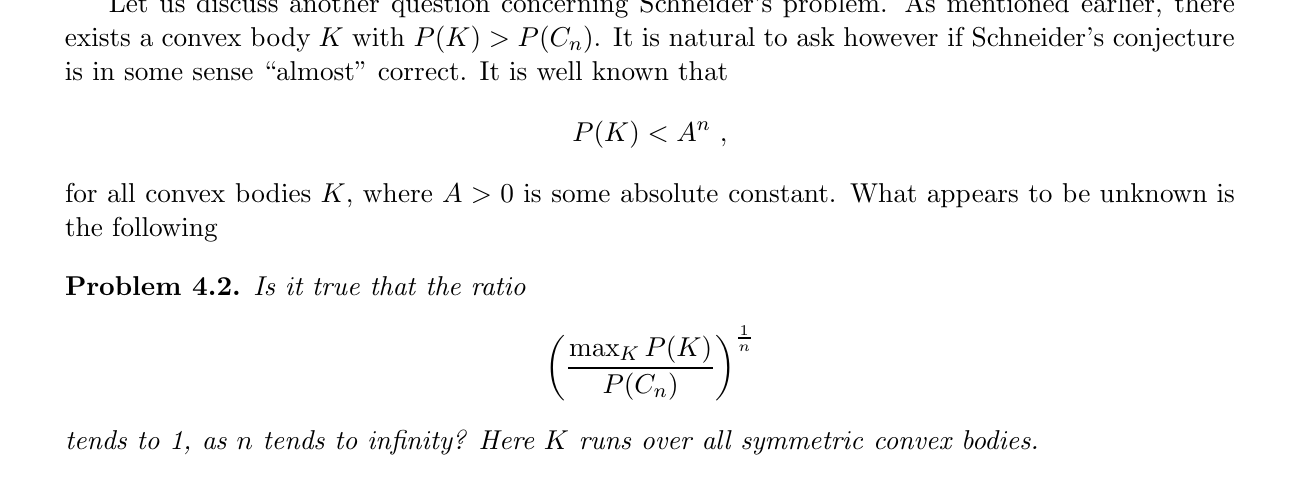
\includegraphics[width=0.96\textwidth]{figures/problem_4_2_crop.png}
\end{center}

Write
\[
 S_n=\sup\{P_n(K):K\subset\R^n\text{ is a centrally symmetric convex body}\}.
\]
Thus the question is whether $(S_n/2^n)^{1/n}\to1$.

\section{Idea of the proof}

The missing operation is Cartesian product.  Cauchy's projection formula
shows that the projection body of $K\times L$ is a correspondingly scaled
Cartesian product of $\Pi K$ and $\Pi L$.  All volume factors cancel in
$P$, making $P$ multiplicative.  Therefore a strict gap in any one fixed
dimension repeats independently in every Cartesian factor and becomes an
exponential gap.

The smallest convenient exact gap is three-dimensional.  The projection
body of the regular octahedron $B_1^3$ is a rhombic dodecahedral zonotope.
Four determinants give its volume as $16$, and hence
$P_3(B_1^3)=16/(4/3)^2=9$.  Cartesian powers compare $9^m$ with the cube's
$8^m$.

\section{Product multiplicativity}

\begin{lemma}[projection body of a product]\label{lem:product}
Let $K\subset\R^a$ and $L\subset\R^b$ be convex bodies, with the two
spaces embedded orthogonally in $\R^{a+b}$.  Then
\begin{equation}\label{eq:pi-product}
 \Pi(K\times L)=|L|\,\Pi K\times |K|\,\Pi L
\end{equation}
and consequently
\begin{equation}\label{eq:p-product}
 P_{a+b}(K\times L)=P_a(K)P_b(L).
\end{equation}
\end{lemma}

\begin{proof}
First suppose that $K$ and $L$ are polytopes.  Every facet of $K\times L$
is either $F\times L$, where $F$ is a facet of $K$, or $K\times G$, where
$G$ is a facet of $L$.  Its outer normal is respectively $(u_F,0)$ or
$(0,u_G)$, and its area is respectively $|L|\,|F|$ or $|K|\,|G|$.
Cauchy's formula therefore gives, for $(x,y)\in\R^a\oplus\R^b$,
\[
 h_{\Pi(K\times L)}(x,y)
 =|L|h_{\Pi K}(x)+|K|h_{\Pi L}(y).
\]
The right side is the support function of the Cartesian product in
\eqref{eq:pi-product}.  Arbitrary convex bodies follow by polytope
approximation and continuity of projection bodies and volume.

Taking $(a+b)$-dimensional volume in \eqref{eq:pi-product} gives
\[
 |\Pi(K\times L)|=|L|^a|K|^b|\Pi K||\Pi L|.
\]
After division by
$|K\times L|^{a+b-1}=|K|^{a+b-1}|L|^{a+b-1}$, the powers of $|K|$ and
$|L|$ cancel exactly, yielding \eqref{eq:p-product}.
\end{proof}

\section{The exact three-dimensional gap}

\begin{lemma}\label{lem:octahedron}
For $O=B_1^3=\operatorname{conv}\{\pm e_1,\pm e_2,\pm e_3\}$,
\[
 |\Pi O|=16,\qquad |O|=\frac43,\qquad P_3(O)=9.
\]
\end{lemma}

\begin{proof}
The eight facets of $O$ are indexed by $s\in\{\pm1\}^3$.  Each has area
$\sqrt3/2$ and outer unit normal $s/\sqrt3$.  Hence Cauchy's formula gives
\[
 h_{\Pi O}(u)=\frac14\sum_{s\in\{\pm1\}^3}|\langle u,s\rangle|
 =\frac12\sum_{j=1}^4|\langle u,v_j\rangle|,
\]
where one may take
\[
 v_1=(1,1,1),\quad v_2=(1,-1,-1),\quad
 v_3=(-1,1,-1),\quad v_4=(-1,-1,1).
\]
Therefore
\[
 \Pi O=\sum_{j=1}^4[-v_j/2,v_j/2].
\]
For a three-dimensional symmetric zonotope
$\sum_j[-g_j,g_j]$, its volume is
$2^3\sum_{i<j<k}|\det(g_i,g_j,g_k)|$; this follows by the standard
dissection into the parallelotopes generated by triples.  Every one of the
four determinants $\det(v_i,v_j,v_k)$ has modulus $4$.  With
$g_j=v_j/2$, each determinant therefore has modulus $4/2^3=1/2$, and
\[
 |\Pi O|=2^3\cdot4\cdot\frac12=16.
\]
Finally, $O$ is the union of eight coordinate tetrahedra of volume $1/6$,
so $|O|=4/3$ and
\[
 P_3(O)=\frac{16}{(4/3)^2}=9.
\]
\end{proof}

\section{Negative answer and existence of the limit}

\begin{theorem}\label{thm:main}
Problem 4.2 has a negative answer.  More precisely, the limit in the
problem exists and
\begin{equation}\label{eq:main}
 \lim_{n\to\infty}\left(\frac{S_n}{2^n}\right)^{1/n}
 \ge \left(\frac98\right)^{1/3}>1.
\end{equation}
\end{theorem}

\begin{proof}
Lemma~\ref{lem:product} and central symmetry of Cartesian products imply
$S_{a+b}\ge S_aS_b$.  Since $P_n(C_n)=2^n$, the sequence
\[
 T_n=\frac{S_n}{2^n}
\]
is supermultiplicative and satisfies $T_n\ge1$.  Thus
$b_n=\log T_n$ is superadditive.  The source records an absolute constant
$A$ with $P_n(K)<A^n$ for every convex body, so $b_n/n$ is bounded above.
Fekete's lemma now yields
\[
 \lim_{n\to\infty}\frac{b_n}{n}=\sup_{n\ge1}\frac{b_n}{n},
 \qquad
 \lim_{n\to\infty}T_n^{1/n}=\sup_{n\ge1}T_n^{1/n}.
\]
By Lemma~\ref{lem:octahedron}, $S_3\ge9$, whereas $P_3(C_3)=8$.
Therefore $T_3\ge9/8$, which proves \eqref{eq:main}.

Equivalently, without invoking the existence upgrade, Lemma~\ref{lem:product}
already gives
\[
 P_{3m}(O^m)=9^m,
 \qquad
 \left(\frac{S_{3m}}{2^{3m}}\right)^{1/(3m)}
 \ge\left(\frac98\right)^{1/3}.
\]
Hence even the subsequence of dimensions divisible by three is uniformly
separated from one.
\end{proof}

\section{Verification, novelty check, and scope}

The companion script \texttt{code/verify\_projection\_product.py} checks
all four determinants exactly over the integers, the zonotope volume
$16$, the octahedron volume $4/3$, the value $P_3(O)=9$, and the finite
Cartesian-power identities.  The script is diagnostic; the proof above is
fully exact and self-contained.

Cheap run-index searches and bounded exact-phrase/topic searches on
13 August 2026 found the source paper and later descriptions of the still
open exact Schneider projection problem, but no cited resolution of
Problem 4.2 or this Cartesian-product amplification.  This is a bounded
novelty check, not a priority claim.

Theorem~\ref{thm:main} settles only the asymptotic Problem 4.2.  It does
not determine $S_n$, classify maximizers, resolve Schneider's exact
projection problem, or settle the distinct polar projection-body Problem
4.5 in the source.

\paragraph{Human-review recommendation.}
Accept as a candidate full counterexample.  The two substantive checks are
the product identity \eqref{eq:pi-product} and the four determinant values
in Lemma~\ref{lem:octahedron}; both are elementary and exact.

\begin{thebibliography}{9}
\bibitem{source}
C.~Saroglou,
\emph{On the equivalence between two problems of asymmetry on convex bodies},
Discrete Comput. Geom. \textbf{54} (2015), 573--585;
arXiv:1311.4955v2, Problem 4.2.
\end{thebibliography}

\end{document}
